\section{Software zu den vorgestellten Verfahren}
Die bisher vorgestellten Verfahren sind in den meisten grösseren Statistikprogrammen bereits integriert oder können als Erweiterung hinzugefügt werden.
Insbesondere wenn es darum geht, verschiedene Verfahren der Modellselektion zu beurteilen, bietet sich R an.

R ist eine frei verfügbare Programmiersprache für statistisches Rechnen \cite{R:core} und setzt momentan den Standard im Bereich der Rechnergestützten Datenanalyse. 
Eine guter Einstieg in R, mit vielen interaktiven Übungen, bietet der Kurs ``tryR''\footnote{http://tryr.codeschool.com} von code school.
Für das tägliche Arbeiten mit R ist  \citeA{R:Teetor:2011a} empfehlenswert.

\subsection{Modellselektion}
Das exhaustive Verfahren wurde im Paket ``leaps'' von \citeA{R:leaps} implementiert. 
Ausgegeben werden kann Mallows's $C_p$, $R^2$ oder auch das adjustierte Bestimmtheitsmass $\bar R^2$.

Die schrittweise Regression ist ein fester Bestandteil von R  und ermöglicht, eine bestehende Gleichung schrittweise vorwärts, rückwärts oder beidseitig zu durchsuchen.
Als Kriterium wird dabei Akaikes Informationskriterium verwendet, da $step(object, ...)$ eine vereinfachte Implementierung der Funktion $stepAIC(object, ...)$  aus dem Paket ``MASS'' darstellt \cite{R:MASS}. 
Ausführlicher werden die kriteriumsbasierenden Verfahren mit R bei \citeA{faraway2002practical} beschrieben.

\subsection{Kreuzvalidierung}
Für die $k$-fache Kreuzvalidierung bietet sich die Funktion $CVlm(...)$ aus dem Paket ``DAAG'' an \cite{R:DAAG}. 
Die Funktion bietet über die reine Berechnung hinaus die Möglichkeit, die $k$ Durchgänge grafisch auszugeben.

\begin{figure}[hbtp]
\centering
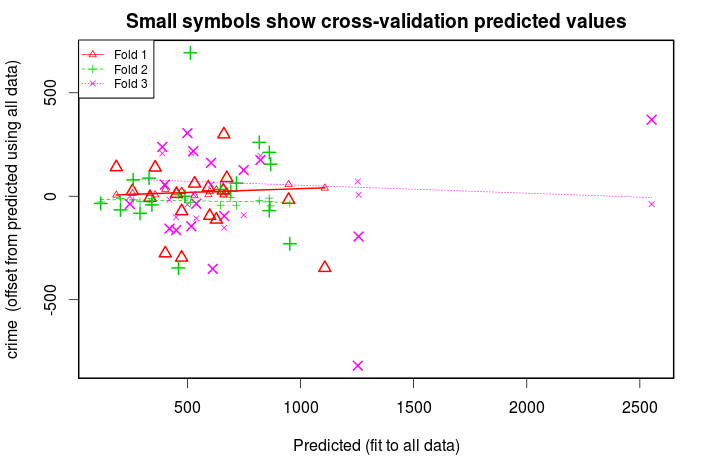
\includegraphics[width=\textwidth]{cvlm.png}
\caption{Residualplot einer 3-fachen Kreuzvalidierung mittels  Die Abszisse beschreibt die vorausgesagten Werte. Auf der Ordinate ist die Abweichung der Vorhersage zum wahren Wert des Kriteriums abgetragen, hier Gewaltdelikte pro 100'000 Einwohner.}
\label{plot:cvlm}
\end{figure}